\documentclass[12pt]{article}
\usepackage[margin=1in]{geometry}
\usepackage[backend=biber, style=numeric-comp, sorting=none]{biblatex}
\usepackage{graphicx}
\usepackage{float}	
\usepackage{hyperref}
\usepackage{enumitem}
\usepackage{rotating}
\addbibresource{references.bib}

\hypersetup{
    colorlinks,
    citecolor=black,
    filecolor=black,
    linkcolor=black,
    urlcolor=black
}

\makeatletter
\renewcommand\paragraph{\@startsection{paragraph}{4}{\z@}%
            {-3.25ex \@plus1ex \@minus.2ex}%
            {1.5ex \@plus.2ex}%
            {\normalfont\normalsize\bfseries}}
\makeatother
\setcounter{secnumdepth}{4}
\setcounter{tocdepth}{4}


\title{RISC-V: A Didactic Platform \\
Report}
\author{Jules PERRIN, Professor: Theo KLUTER}
\date{\today}

\begin{document}
\maketitle
\tableofcontents

\section{Introduction}
\subsection{Motivation}
This project, RISC-V: A Didactic Platform, embarks on the pursuit of simplifying complex computer architecture concepts, 
targeting an academic audience who is striving to comprehend the intricate world of processor design. 
It specifically focuses on the creation of a RV32I processor, based on the RISC-V instruction set architecture.

RISC-V, an open standard instruction set architecture (ISA), has increasingly gained popularity due to its simplified design and 
flexibility for customization. While its usage has been witnessed across a multitude of applications, its potential as an educational tool remains largely unexplored. 
The objective of this project is to bridge this gap by providing a detailed, comprehensible, and implementable design of an RV32IM processor, leveraging the RISC-V architecture.

This project not only contributes to the existing body of knowledge around RISC-V and processor design but also aims to democratize access to information on complex computing architectures. 
Through this platform, users will not only learn the theory behind processor design but will also gain valuable hands-on experience with the actual implementation, 
enabling them to better understand the interplay between hardware and software in a computing system.

In an era where the understanding of computer architecture is pivotal for both hardware and software development, 
a project like RISC-V: A Didactic Platform can serve as a crucial resource. 
By harnessing the power of the RISC-V architecture and presenting it through a user-friendly and accessible platform, 
we hope to elevate the understanding of processor design to new heights.
\subsection{Project Scope}
Here are the different main focus points of the project:


\begin{enumerate}[label={\textbullet}]
    \item Openess: It is an important point for the project to use as much as possible
    open source software and also for the project to be as open as possible such that people 
    can work on it with the less possible restrictions.
    \item Comprehensive: Since the project needs to be open source and be used by academic people
    to understand but also add things on top of it, the project needs to focus on being as comprehensive 
    as possible.
    \item Simplicity: This point is linked a bit with the last one, but the project doesn't aim as 
    performance first, but more as ease of understanding, so if a solution can be easier but degrade 
    a bit the performance, it should be taken except if it adds an educational value to do it
\end{enumerate}
\subsection{Project Objectives}

Overall, the project aims to give a very basic implementation of an RV32IM processor such 
that it can be used as an academic tool to teach and explain how a RISC processor works 
and how to build one using HDL languages such as Verilog. Here are the main objectives that 
has been set for the project:

\begin{enumerate}[label={\textbullet}]
    \item First create an unpipelined version of the RV32IM processor as a proof of concept
    \item Pipeline the existing unpipelined version of the processor
    \item Fix the different issues caused by the pipelining of the processor, mainly the 
    data dependency but also the branch prediction problem by either stall or implementing some 
    forwarding paths and branch predictor and mechanisms to make everything work correctly
    \item The simulation should works on Icarus Verilog to make the whole process more open instead 
    of relying on proprietary software such as Questa Modelsim.
    \item Add extensive testing of the different main modules to make the processor as reliable 
    as possible.
    \item Add an easy way for users to create programs and load them into the ROM memory.
    \item Document everything such that users can easily understand how things work and can 
    work on it easily.
\end{enumerate}

\section{Background Research and Knowledge}
\subsection{RISC-V}
RISC-V is an open-source instruction set architecture (ISA) based on the reduced instruction set
computer (RISC) principles. It is a free and open ISA enabling a new era of processor innovation
through open standard collaboration.

Most of the research I've done on it to understand how it works and how to implement it has been
done on the official website of the RISC-V foundation~\cite[p.~9-25]{riscv_manual} and of course more precisely
the chapter about the RV32I base integer instruction set. Inside it describes how the different instructions
are encoded with the 6 different formats~\cite[p.~104-105]{riscv_manual} that are used to encode the different instructions but also 
how the different instructions should behave using a mix of the manual but also a reference card~\cite[p.~81-83]{refcard}.
\subsection{Architecture}
\subsubsection{Unpipeline}
The unpipelined version of the CPU is mostly inspired by the one we did during the Comparch 1-2
courses at EPFL since NiosII and RISC-V are very similar. The main difference is that the RISC-V
is a 32 bits architecture while NiosII is a 16 bits architecture and also that RISC-V has a lot more
instructions than NiosII with small differences in how they work. 

\subsubsection{Pipeline}
The pipelined version is inspired also mostly by what we did during the Comparch 2 course at EPFL but
since we didn't implement the branch predictor and the forwarding paths, I had to imagine and think about 
most of the implementation myself. I've only done a couple of research to see if I could find some examples of 
such implementation mostly about forwarding paths since I wasn't sure how to implement it correctly at first 
glance. I've used mainly this pdf~\cite{forwarding_paths} to reassure myself that I was doing it correctly.
The branch predictor part has an algorithm I haven't invented called a two-level adaptive branch predictor~\cite{two_level_adaptive}.
It uses a 2 bits saturating counter but also knows patterns such that the predictions apply locally to the 
branch. It is a very simple algorithm but it works well enough for this project.
\subsection{Verilog}
Not knowing anything about Verilog since at EPFL we used VHDL instead, I had to learn it from scratch.
For that, I've used a website given by the professor~\cite{verilog_tutorial} that explains the basics of Verilog and how to use it.
From here I've started creating small modules and searching for examples on the internet to see how other people were doing it
and also when needed I've used different forums to find answers to my questions and when needed consulted the official 
Verilog documentation~\cite{verilog_doc}.
\subsection{Simulation Tools}
During the project, I mainly used a close source simulator that we were using at EPFL and 
developed by Intel called Questa Modelsim. It is a great tool combining compiling and seeing 
the waveforms of the signals in the same window. It is also very easy to use and has a lot of
features that I haven't used during the project. The only downside is that it is not free and
it is quite buggy sometimes and you need to activate an option called \texttt{full visibilty}
to have access to all the signals in the waveform window. At the end of the project, since I had 
to implement the CI, I needed a free simulator with a command line interface and I've used
Icarus Verilog. It is a free simulator that is not too hard to use and has a command-line interface.
The only downsides I've found while using it are that there is not a lot of documentation~\cite{icarus_tutorial} 
and it is a bit less user-friendly than Questa Modelsim. You have to use a different tool to see the waveforms
like GTKWave and you don't have access to the array of signals easily like in Questa Modelsim.
Also, one weird issue I've encountered is that the simulation gives different results than Questa Modelsim
because the full visibility option does things differently than Icarus Verilog, but I've luckily
found the issue even though to this day I don't know why it was doing that.
\subsection{RISC-V Toolchain}
\subsubsection{Developping using Assembly Code}
It is not that easy to find a way to compile a RISC-V RV32I assembly code into a hexadecimal file 
that can be read by the ROM module. So for that, I've found two projects that helped me 
develop simple programs for testing purposes. The first one is a Python script that converts
pseudo instructions into hexadecimal instructions~\cite{riscv_python_assembler}. The second one is a
website that converts assembly code into hexadecimal instructions~\cite{riscv_online_assembler}.
One last tool I've used to reverse the hexadecimal instructions into assembly code is a website~\cite{riscv_online_encoder_decoder} but 
also used it to modify one instruction at a time to see what it does.

\subsubsection{RISC-V GNU Compiler Toolchain}
The RISC-V GNU Compiler Toolchain is a set of tools that allows you to compile C/C++ code into
RISC-V assembly code. It is composed of a compiler, an assembler, a linker and a debugger. To use it 
you need to compile it from the source code which was not that easy to do because the documentation for
such a small architecture set is not that great and since we're developing bare metal programs, it is even
harder to find information about it. So I've used the official documentation~\cite{riscv_gnu_toolchain} and
also a tutorial I've found on the internet~\cite{riscv_gnu_toolchain_baremetal_tutorials} to compile it and finally use 
it.

\section{Design}
All the different constants were used in the project such that the different values linked to the different operators for 
the LSU, BRU and ALU. It is not an ideal solution but since Verilog doesn't have a better way to share 
constants by for example doing enums, I decided to do it this way. So all the constants are in the parameters.vh file inside 
the Verilog directory.
\subsection{Unpipelined Design}
The first step in the project other than learning how to develop in Verilog was to create an unpipelined version of the intended processor.
This version is quite more simple than the pipelined version as it doesn't have to deal with the hazards that can occur in a pipelined and 
issues with branches and jumps but also because it doesn't need any pipeline registers in between the different stages. I will give you an 
overall view of the design without the details of each connection between the different modules since it is not the main focus of this project 
and was more of a way to learn how to use Verilog and the tools associated with it but also a temporary step before the pipelined version.

\begin{figure}[H]
    \centering
    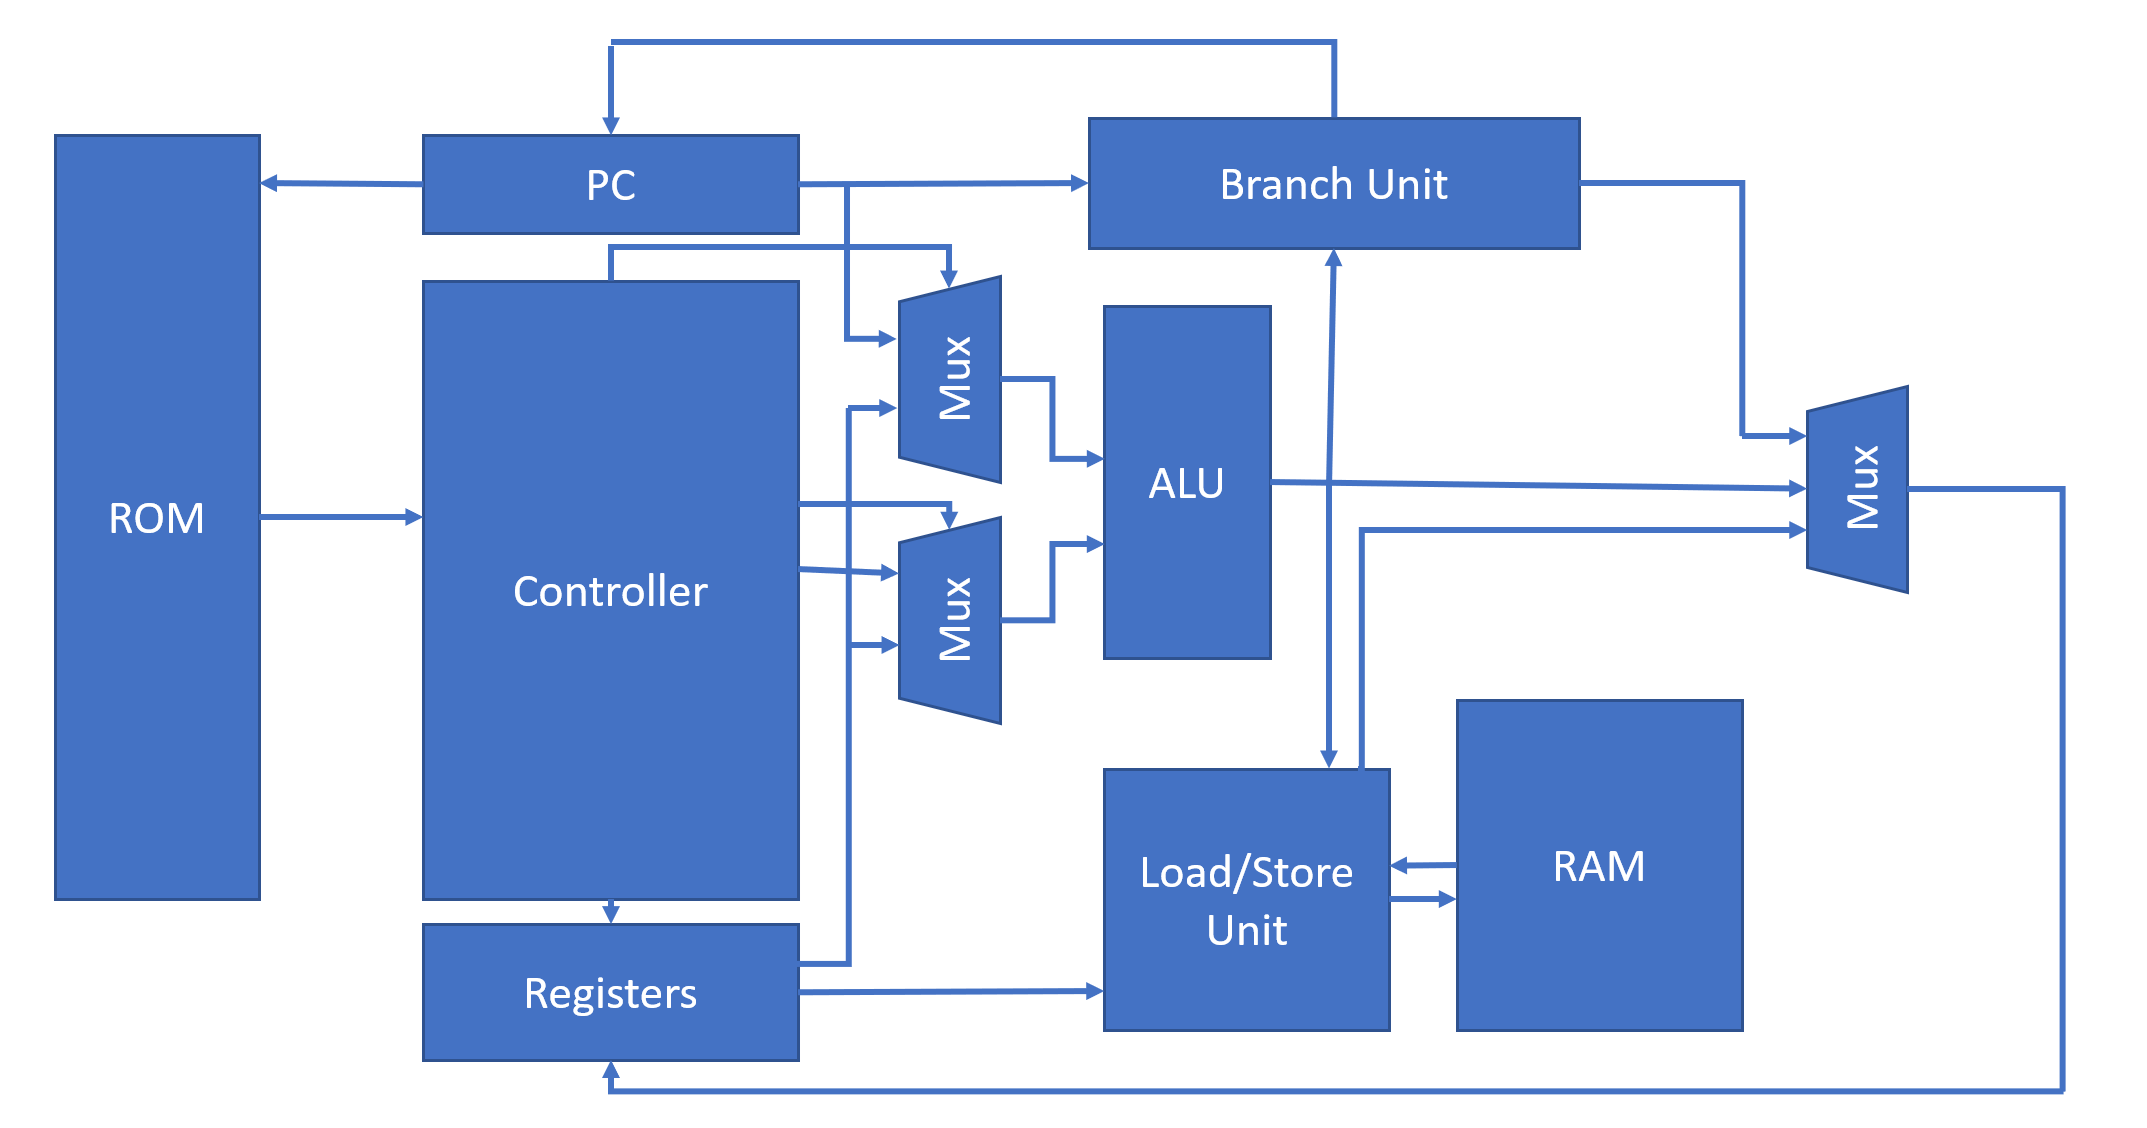
\includegraphics[width=0.85\textwidth]{design/unpipelined/images/unpipelined_cpu.png}
    \caption{Unpipelined CPU design}
    \label{fig:unpipelined_cpu_design}
\end{figure}

I will not go into the details of each module since it will be done in the next section about the pipelined version but I will give you a
brief overview of how the unpipelined version works.
First, the instruction is loaded from the ROM using the address given by the PC (Program Counter). Then the instruction needs to be decoded to know 
what it does and what are the operands and that's the job of the Controller that will try to match the different types of instruction to finally 
find the right one. Once it is done, it will output the different control signals to the register file, the ALU, the branch unit and the load/store unit such 
that it executes the instruction correctly with the correct data. The role of the ALU (Arithmetic Logic Unit) is to execute the different arithmetic
and logic operations such as addition, subtraction, multiplication, division, bitwise operations, etc. In the case of a branch instruction, the branch unit
will check if the instruction is a conditional one or not. In case it is one then it uses the result of the ALU to check if the condition is true or not
and update the PC accordingly. Finally, the load/store unit will load or store data from or to the RAM depending on the instruction. It is also using the 
result of the ALU since we can offset the address by an immediate value and that needs to be done by the ALU\@.
At the end of the cycle, a MUX will select among the three different results (ALU, branch unit and load/store unit) the one that will be written to the register file
according of course to the instruction executed.
Everything is done in one cycle and the next instruction is loaded from the ROM and the process starts again. \\

As we can see, the unpipelined version is quite simple then why do we need to pipeline it? The answer is performance. Indeed, the unpipelined version
is quite slow since it needs to wait for the instruction to be executed before loading the next one. But that can be improved by pipelining the processor
that will divide the execution of an instruction into multiple stages and execute multiple instructions at the same time and that's what we will see in the next section.


\subsection{Pipelined Design}
So what is the purpose of a Pipelined version of a CPU\@? As stated in the previous section, the unpipelined version is quite slow since it needs to wait for the instruction to be executed before loading the next one. 
Pipelining follows the idea of dividing the work among smaller parts and executing them in parallel. In the case of a CPU, it means that we will divide the execution of an instruction into multiple stages and execute multiple instructions at the same time.
Since each part has a smaller quantity of work to do, we can hopefully increase the clock frequency and thus obtaining in average a better throughput resulting in better performance.

\begin{figure}[H]
    \centering
    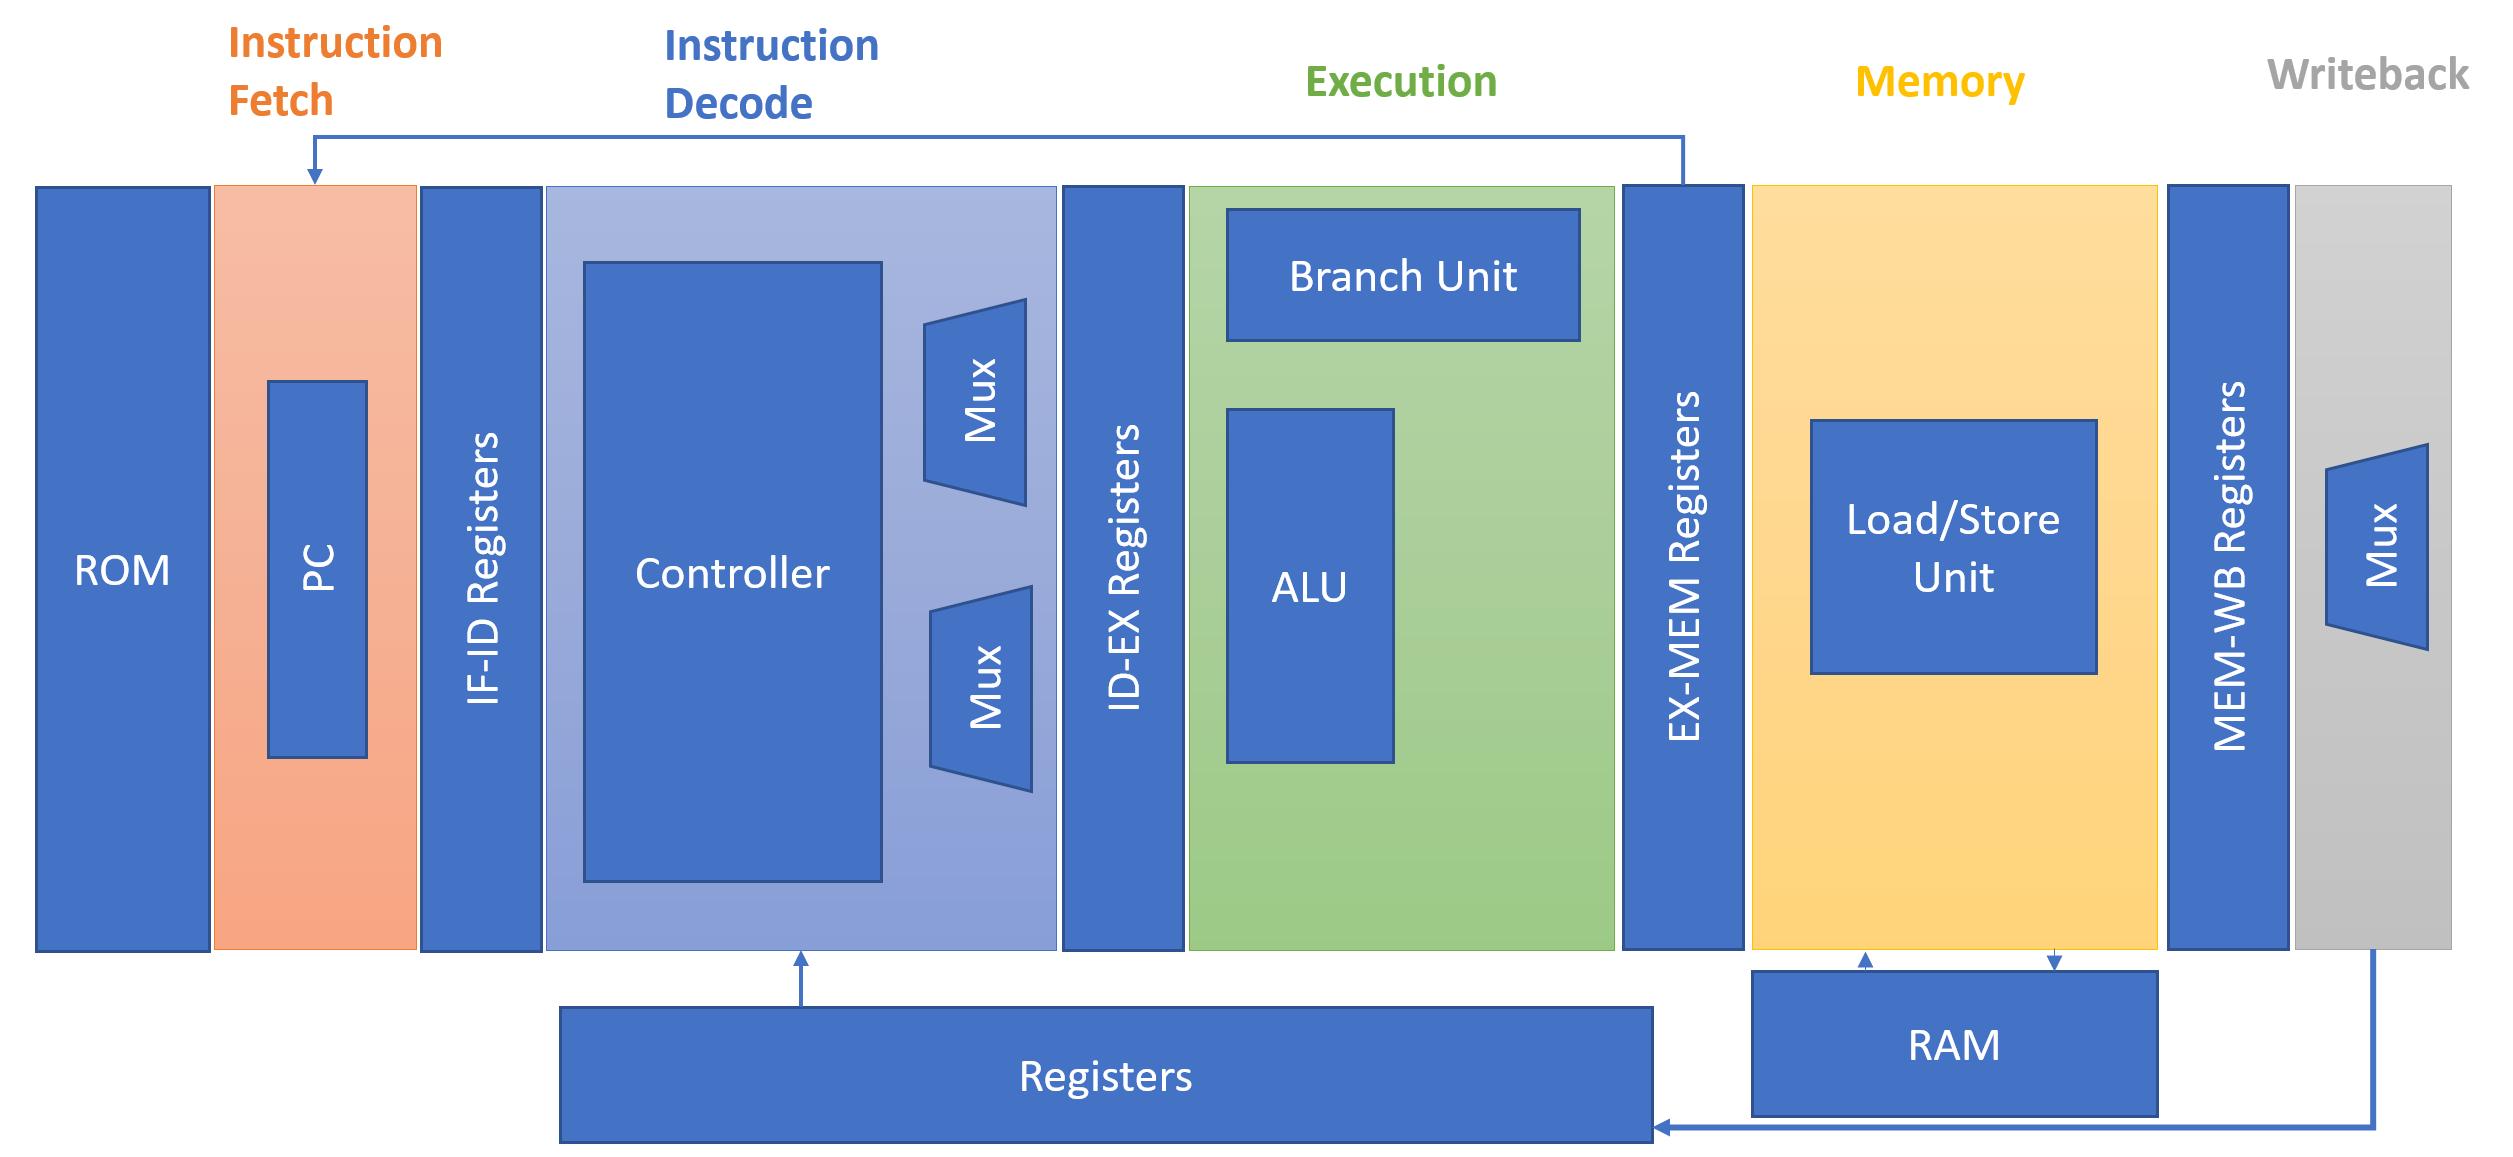
\includegraphics[width=1\textwidth]{design/pipelined/images/pipelined_design.png}
    \caption{Pipelined CPU design}
    \label{fig:pipelined_cpu_design}
\end{figure}

So here is the idea, we will divide the execution of instruction into five stages: Instruction Fetch (IF), Instruction Decode (ID), Execute (EX), Memory (MEM) and Write Back (WB).
Each stage will be executed in parallel and will be connected to the next one using pipeline registers. The pipeline registers are used to store the data between each stage and are synchronized with the clock.
The IF stage will fetch the instruction from the ROM using the PC (Program Counter) and will send it to the ID stage. The ID stage will decode the instruction and send the control signals to the different units 
(ALU, Branch Unit, Load/Store Unit) and will also send the operands to the EX stage. The EX stage will execute the instruction and send the result to the MEM stage. 
The MEM stage will load or store data from or to the RAM and send the result to the WB stage. Finally, the WB stage will write the result to the register file. \\

But for the most attentive reader or anybody with a bit of experience in computer architecture, you may have noticed that there is a problem with this design. 
This design will lead so some issues in two different ways. 

\begin{enumerate}[label=\textbullet]
    \item The first one is that since instruction is not executed anymore in one cycle, its result will not be available in the next cycle.
    This is an issue because if the next instruction depends on the result of the previous one, it will not be able to execute correctly and will use 
    outdated data from the registers. This is called a \textbf{Data Hazard}.
    \item The second one is related to the branching mechanism, since the result of the branch will be available only after the EX stage, the PC will not be updated
    before that leading to possible wrong instructions being fetched and executed in the pipeline. This is called a \textbf{Control Hazard}.
\end{enumerate}

For resolving these two issues we have two solutions. Either stalling the pipeline when a hazard is occurring or when a branch is detected at the IF stage such that we wait for 
the result before fetching any new instruction. One issue with this approach is of course performance which is unfortunate since the main purpose of pipelining is to improve performance.

Another solution for the data hazard is to use \textbf{Forwarding} which consists of forwarding the result of the ALU to the EX stage and the result of the MEM stage to the EX and MEM stages.
The only moment we will have to stall the pipeline is when we have a load instruction followed by an instruction using the result of the load. In this case, we will have to stall the pipeline
for one cycle to wait for the result of the load.

\begin{figure}[H]
    \centering
    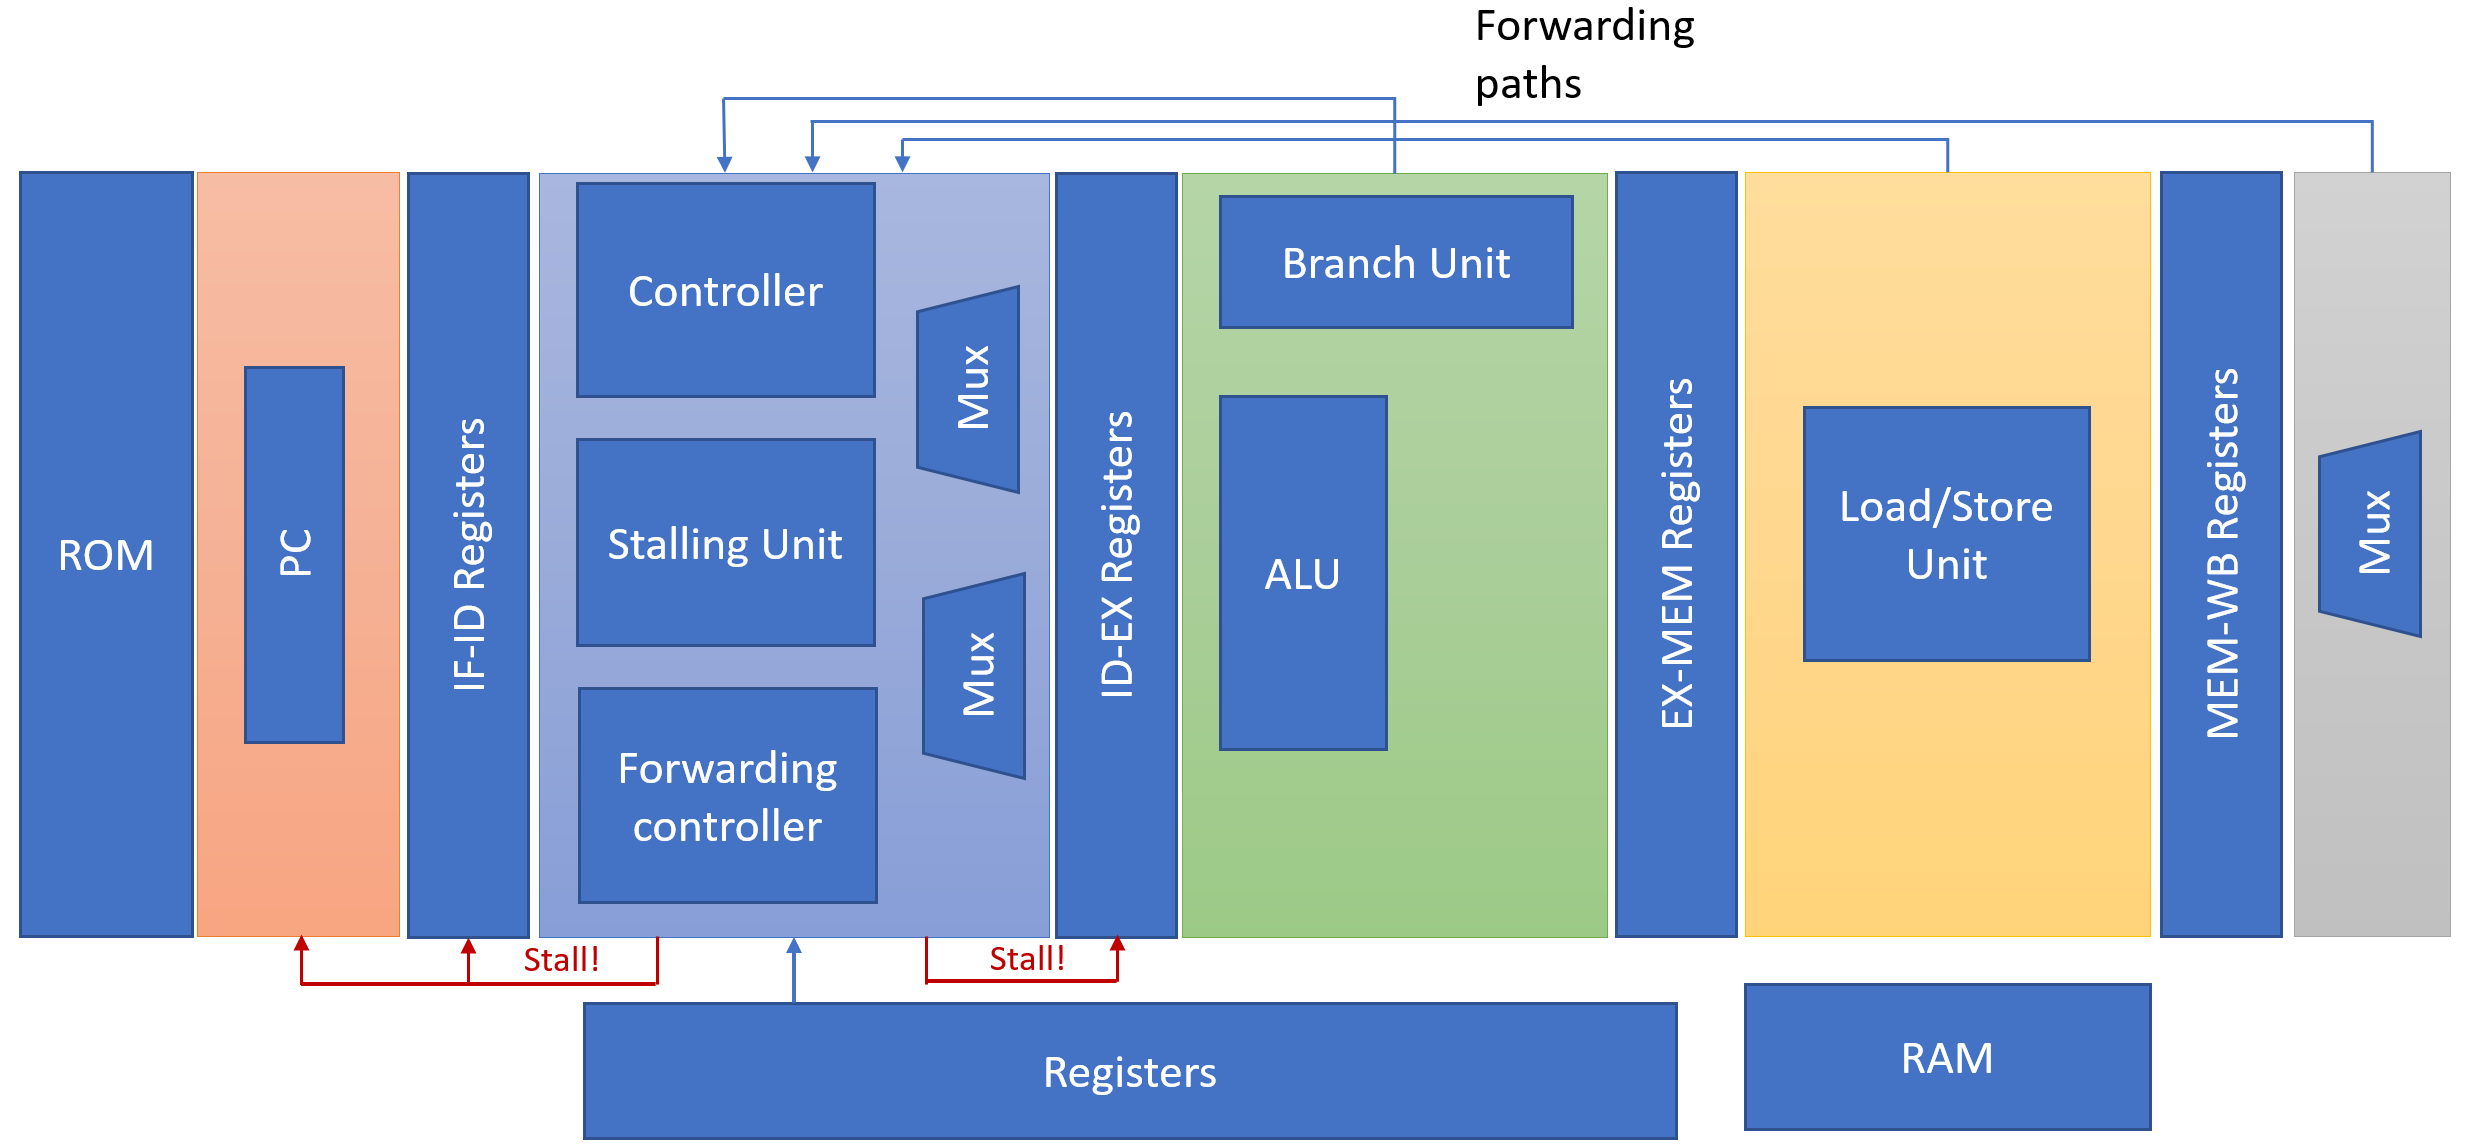
\includegraphics[width=1\textwidth]{design/pipelined/images/pipelined_design_forwarding.png}
    \caption{Pipelined CPU design with forwarding paths}
    \label{fig:pipelined_cpu_design_forwarding}
\end{figure}

Another solution for the control hazard is to use \textbf{Branch Prediction} which consists of predicting the result of the branch and fetching the instruction at the predicted address.
It is not always possible to predict correctly the result of a branch but it is possible to use some heuristics to improve the prediction accuracy. For example, we can predict that a branch will not be taken
if the previous branch was not taken. This is called a \textbf{Branch Not Taken} heuristic. Another heuristic is to predict that a branch will be taken if the previous branch was taken. This is called a \textbf{Branch Taken} heuristic.
Of course, you can develop more complex heuristics but this is out of the scope of this project and I invite you to use the link in the reference to the given algorithm I've chosen 
to implement in the CPU\@. But when the prediction is wrong, we will have to flush the pipeline and restart the execution from the correct address. \\

\begin{figure}[H]
    \centering
    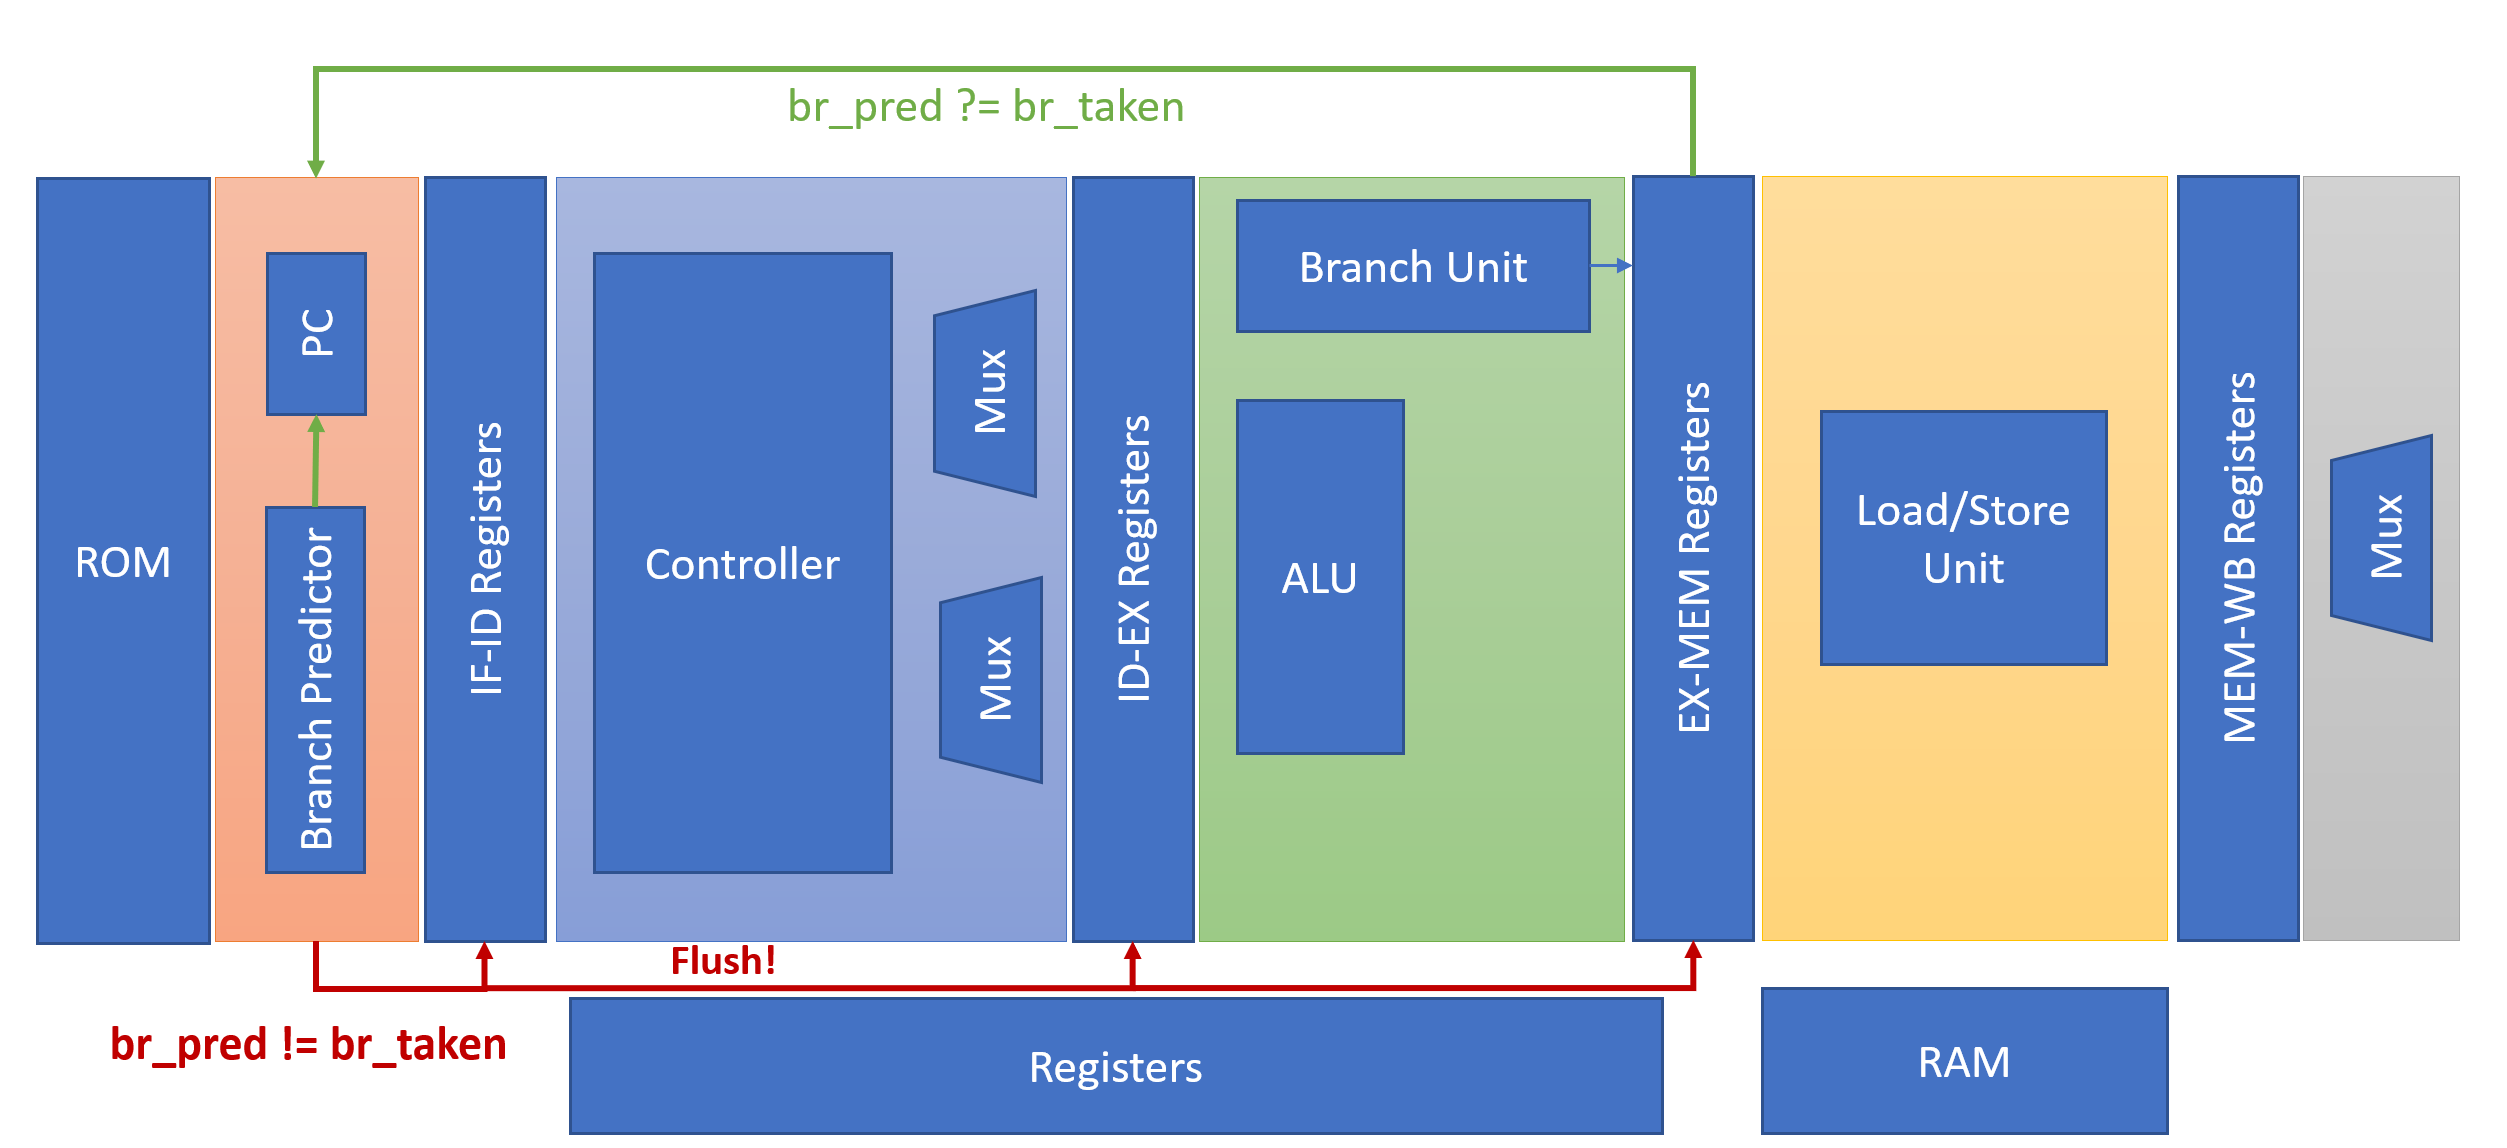
\includegraphics[width=1\textwidth]{design/pipelined/images/pipelined_design_predictor.png}
    \caption{Pipelined CPU design with branch predictor}
    \label{fig:pipelined_cpu_design_predictor}
\end{figure}






\printbibliography[heading=bibintoc]

\appendix
\section{Detailed Pipelined CPU Design}
\label{appendix:pipelined_design}
\begin{sidewaysfigure}
    \centering
    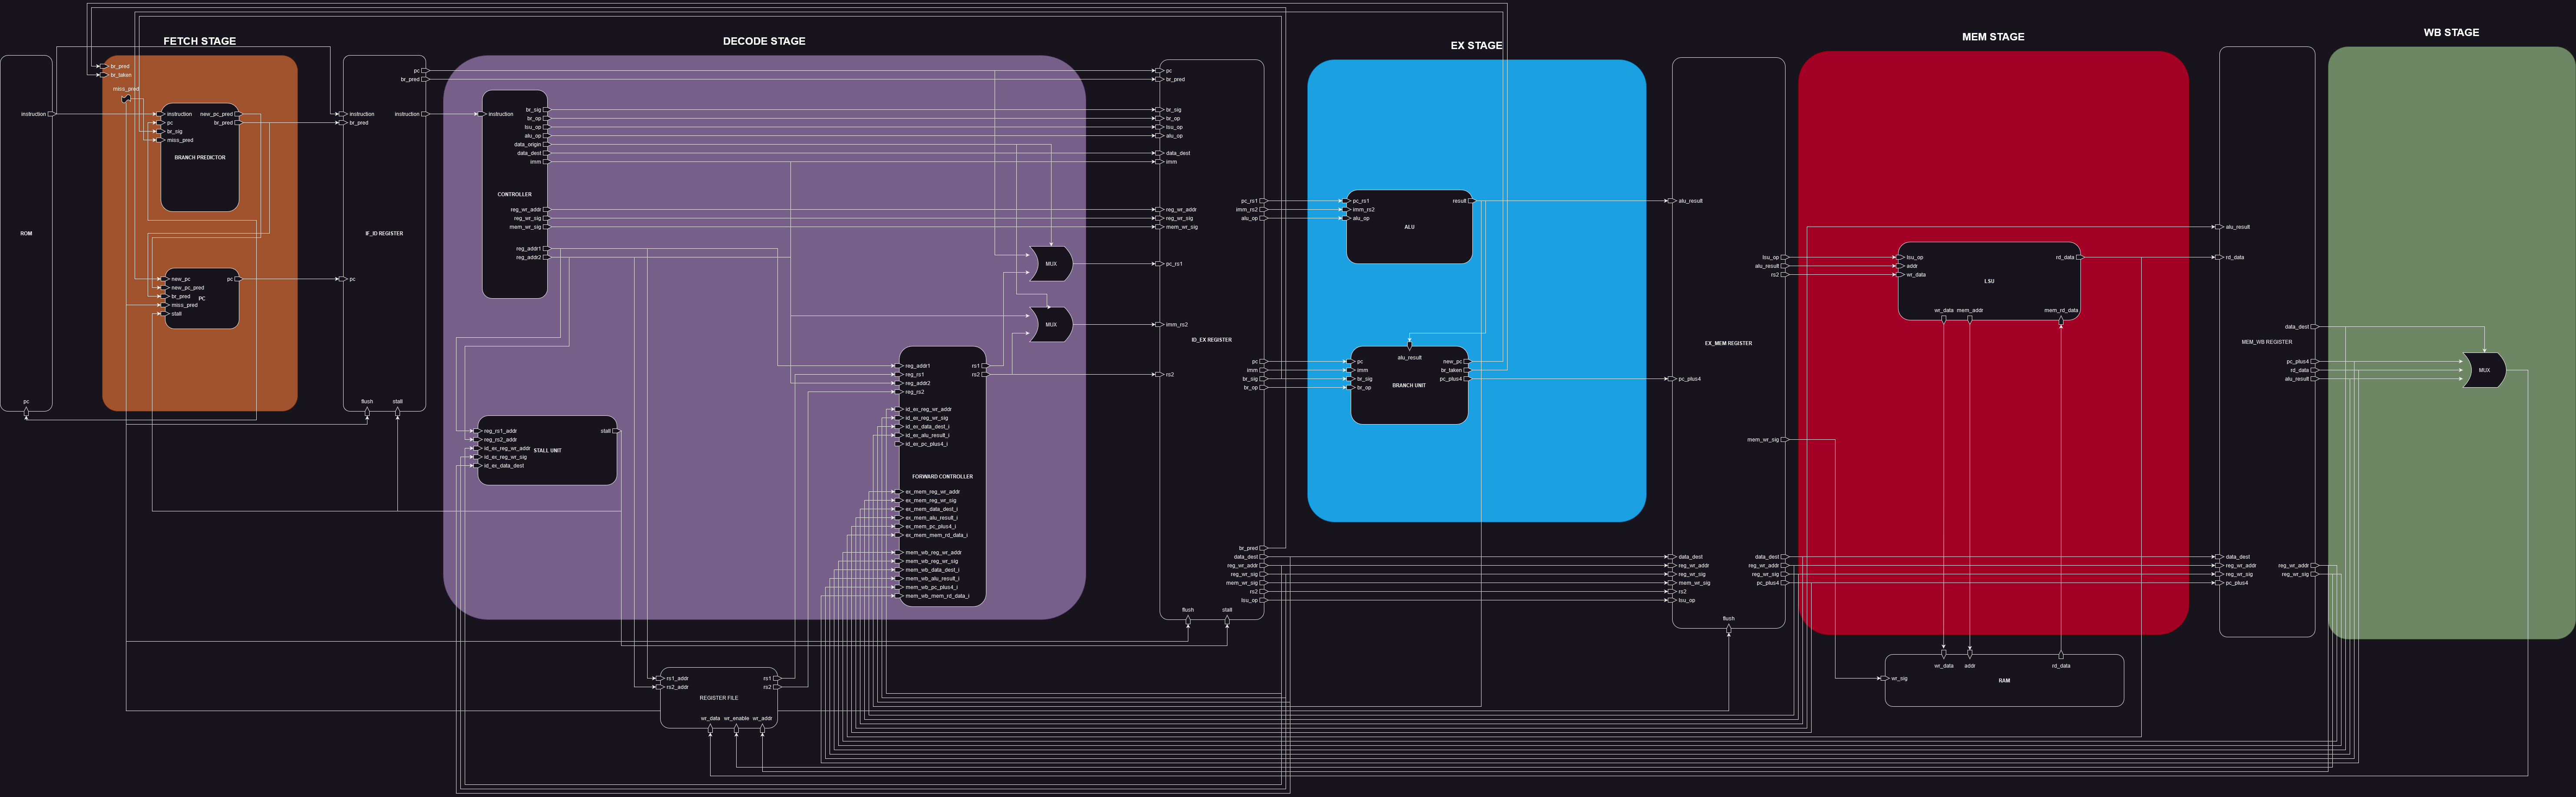
\includegraphics[width=\textheight]{appendix/images/pipelined_design_detail.png} % Note the change in width to \textheight
    \caption{Detailed Pipelined CPU Design}
\end{sidewaysfigure}
\end{document}
